%File: formatting-instruction.tex
\documentclass[letterpaper]{article}
\usepackage{url,graphicx,xcolor}
\usepackage{amsmath}
\usepackage{times}
\usepackage{helvet}
\usepackage{courier}
\usepackage[]{faikrmod3} % without guidelines
\frenchspacing
\setlength{\pdfpagewidth}{8.5in}
\setlength{\pdfpageheight}{11in}

\pdfinfo{
/Title (Predicting Spotify Track Popularity through Bayesian Reasoning)
/Author (Mattia Semproli)}
\setcounter{secnumdepth}{0}
 \begin{document}

\title{Predicting Spotify Track Popularity through Bayesian Reasoning}
\author{Mattia Semproli \\
Master's Degree in Artificial Intelligence, University of Bologna\\
mattia.semproli2@studio.unibo.it
}
\maketitle

\begin{abstract}
\begin{quote}
This mini-project applies Bayesian Networks to the problem of understanding
what drives the popularity of a music track. We build a small, custom-defined
Discrete Bayesian Network over seven variables derived from the Spotify Tracks
Dataset (genre, tempo, danceability, energy, valence, explicit content, and
popularity), fit its parameters via Maximum Likelihood Estimation, and use
exact inference to answer three concrete questions about track popularity.
We find that energy is a considerably stronger driver of predicted
popularity than mood (valence), and that genre alone produces large shifts
in the odds of a track being popular.
\end{quote}
\end{abstract}


\section{Introduction}
\subsection{Domain}
Streaming platforms such as Spotify expose, for each track, audio features
computed from the signal itself (danceability, energy, valence, tempo,
etc.) together with a popularity score. This project models the
probabilistic relationships between a track's genre, tempo, audio
characteristics, and resulting popularity, using the Spotify Tracks
Dataset~\cite{spotify-dataset}.

\subsection{Aim}
The purpose of this project is to build a Bayesian Network relating a
track's genre, tempo and audio characteristics to its popularity, and to
use it to answer the following questions:
\begin{itemize}
    \item Does genre alone shift the odds of a track being popular?
    \item Does a track's mood (valence) matter more than its energy for
    predicting popularity?
    \item Do audio features depend on each other beyond what genre alone
    explains (e.g.\ does tempo drive energy, which drives mood)?
    \item How large a swing in predicted popularity can be produced by
    combining favorable vs.\ unfavorable evidence across all features?
\end{itemize}

\subsection{Method}
We model the problem with a \textbf{Discrete Bayesian Network}: a directed
acyclic graph (DAG) in which each node is a categorical random variable
(a finite number of possible states, no continuous values) and each
node's distribution is conditioned only on its parents in the graph. We
used the pgmpy library to define this DAG manually (structure not learned
from data) and to fit its Conditional Probability Tables (CPTs) via
Maximum Likelihood Estimation. We then used Variable Elimination to
perform exact inference and answer the questions above.

\subsection{Results}
The clearest single driver is energy, not mood or genre in isolation.
Classical and jazz stand out as weaker performers; combining several
favorable features at once produces a much larger swing in predicted
popularity than any single feature alone.

\section{Model}

\begin{figure}[h]
    \centering
    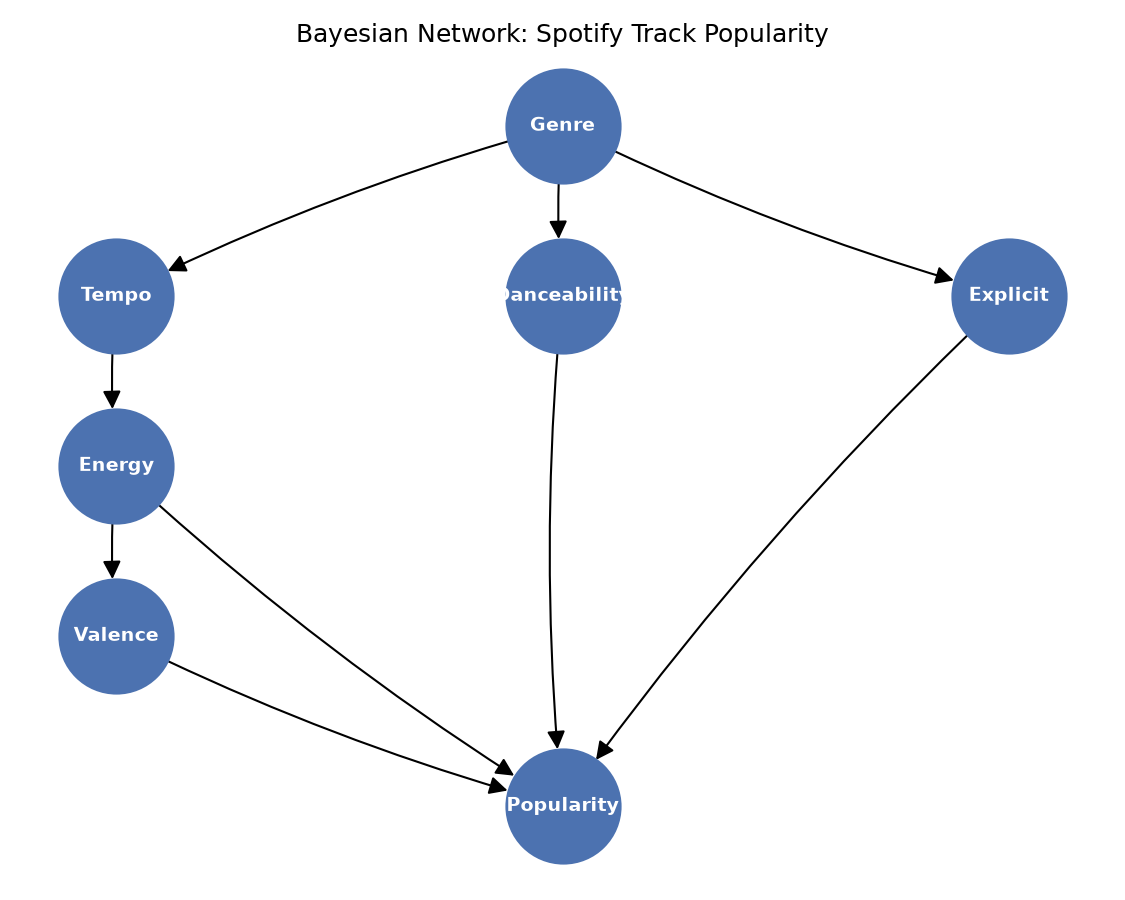
\includegraphics[width=0.9\columnwidth]{network_diagram.png}
    \caption{The custom Bayesian Network relating genre and audio features
    to track popularity.}
    \label{fig:network}
\end{figure}

The dataset was restricted to 6000 tracks evenly split across six genres
(pop, classical, jazz, metal, edm, hip-hop), chosen to span a wide range of
average popularity and musical style while keeping the model small and the
CPTs well estimated. Continuous audio features (danceability, energy,
valence, tempo) and the popularity score were discretized into three bins
each using fixed range cuts (rather than quantile-based cuts, since
popularity is heavily skewed towards zero and quantile binning produced
degenerate bins). The seven nodes are:
\begin{itemize}
    \item \textbf{Genre}: one of the six chosen genres.
    \item \textbf{Tempo}: slow/medium/fast (bpm-based).
    \item \textbf{Danceability}, \textbf{Energy}: low/med/high, derived from
    Spotify's own 0--1 audio feature scores.
    \item \textbf{Valence}: sad/neutral/happy, Spotify's measure of musical
    mood/positiveness.
    \item \textbf{Explicit}: boolean flag for explicit content.
    \item \textbf{Popularity}: low/med/high (target node).
\end{itemize}

A structure where Genre is the sole cause of every audio feature, with all
features feeding directly into Popularity, would assume that once Genre
is known, the audio features are mutually independent -- unrealistic:
slow tracks are low-energy 47\% of the time vs.\ 19\% for fast tracks, and
low-energy tracks are ``sad'' 51\% of the time vs.\ 13\% ``happy''. We
therefore modeled these dependencies explicitly with \textbf{Genre
$\rightarrow$ Tempo $\rightarrow$ Energy $\rightarrow$ Valence}, alongside
Genre's direct influence on Danceability and Explicit, with all four
audio/content features feeding into Popularity. Popularity's parent set
has only these four direct parents, keeping its CPT size and
data-sufficiency manageable (47/54 parent combinations present, minimum
count 1); the two additional CPTs (Energy$\mid$Tempo, Valence$\mid$Energy)
are fully populated (9/9 combinations each, minimum count $>$175).

\section{Analysis}

\subsection{Experimental setup}
We ran four sets of exact-inference queries using Variable Elimination:
(1) $P(\text{Popularity} \mid \text{Genre} = g)$, where $g$ ranges over
the six genres, with no other evidence; (2) $P(\text{Popularity} =
\text{high} \mid \text{Valence} = v)$ and $P(\text{Popularity} =
\text{high} \mid \text{Energy} = e)$, where $v \in \{\text{sad},
\text{neutral}, \text{happy}\}$ and $e \in \{\text{low}, \text{med},
\text{high}\}$, to compare the two features' individual effect on
popularity; (3) a best-case scenario (pop, high danceability, high energy,
happy, non-explicit) versus a worst-case scenario (classical, low
danceability, low energy, sad, non-explicit); (4) $P(\text{Popularity} =
\text{high} \mid \text{Tempo} = t)$, where $t \in \{\text{slow},
\text{medium}, \text{fast}\}$, testing whether tempo shifts popularity
odds through its effect on energy.

\subsection{Results}
\textbf{Genre.} Classical (50.6\% low popularity, 17.8\% high) is the
weakest genre for popularity, while hip-hop/edm/metal do best (24--28\%
high) -- part of genre's effect is mediated through the
Tempo$\rightarrow$Energy$\rightarrow$Valence chain rather than acting
directly on every feature.

\textbf{Valence vs.\ energy.} Energy shows a clear, monotonic effect:
P(high popularity) rises from 12.6\% (low) to 24.8\% (medium) to 27.9\%
(high). Valence has a small, non-monotonic effect (25.3\% / 24.7\% / 18.3\%
for sad / neutral / happy) -- energy is clearly the dominant driver of the
two.

\textbf{Tempo.} Slow tracks are noticeably less likely to be highly popular
(18.0\%) than medium (24.7\%) or fast (24.3\%) tracks, consistent with slow
tracks tending toward lower energy -- itself the strongest direct driver
of popularity. Tempo's own effect on popularity, in other words, runs
mainly through energy, matching what the structure assumes.

\textbf{Combined scenarios.} Best-case yields 21.7\% chance of high
popularity (43.7\% low, 34.6\% med) vs.\ 2.5\% for worst-case (88.8\% low)
-- essentially unchanged from a Genre-only structure, since these
scenarios directly fix Danceability/Energy/Valence.

\textbf{Diagnostic reasoning.} We also ran a diagnostic (bottom-up) query,
$P(\text{Genre} \mid \text{Popularity})$: given high popularity, classical
drops to 12.7\% (vs.\ 18.4\% given low popularity), while hip-hop rises to
20.0\% (vs.\ 15.5\%) -- confirming the network reasons correctly from
effect back to cause.

Popularity's parent set -- Danceability, Energy, Valence, Explicit --
implies Genre is d-separated from Popularity given these four features
(genre affects popularity only \emph{through} the audio features it tends
to produce, not directly), and the Tempo$\rightarrow$Energy$\rightarrow$
Valence chain implies Genre is d-separated from Valence given Energy
alone. We verified both hold via exact reachability analysis; both are
structural properties of the DAG we chose, reflecting modeling
assumptions, not discovered facts.

\section{Conclusion}
The main takeaway is that lifestyle/production factors captured by audio
features -- particularly energy -- outweigh a track's genre label as a
driver of predicted popularity, and that modeling dependencies \emph{among}
those features (rather than treating them as independent given genre)
changes which pathways carry that influence, without costing us any
data-sufficiency for the target node. The main limitations are the
discretization of continuous features into only three bins each; the
restriction to six genres out of 114, for tractability; the network
structure being chosen from domain intuition and confirmed correlations
rather than formal structure-learning or independence testing; Maximum
Likelihood Estimation falling back to a uniform distribution for the few
parent combinations absent from our sample, rather than a
Dirichlet-smoothed estimate; and the source dataset's exactly-1000-per-genre
sampling, which gives Popularity's Genre prior an artificial uniformity
not reflective of real-world catalog proportions.


\section{Links to external resources}
\begin{itemize}
    \item Dataset: \url{https://www.kaggle.com/datasets/maharshipandya/-spotify-tracks-dataset}
    \item Code repository: \url{https://github.com/MattiaSemproli/Spotify-Bayesian-Network.git}
\end{itemize}

\bigskip

\bibliographystyle{aaai}
\bibliography{faikrmod3}


\end{document}
